\chapter{}

Existen varias normas para la citación bibliográfica. Algunas áreas del conocimiento prefieren normas específicas para citar las referencias bibliográficas en el texto y escribir la lista de bibliografía al final de los documentos. Esta plantilla brinda la libertad para que el autor de la tesis utilice la norma bibliográfica común para su disciplina. Sin embargo, se solicita que la norma seleccionada se utilice con rigurosidad, sin olvidar referenciar “todos” los elementos tomados de otras fuentes (referencias bibliográficas, patentes consultadas, software empleado en el manuscrito, en el tratamiento a los datos y resultados del trabajo, consultas a personas (expertos o público general), entre otros).

\section{Ejemplos de citaciones bibliográficas}

Existen algunos ejemplos para la citación bibliográfica, por ejemplo, Microsoft Word (versiones posteriores al 2006), en el  menú de referencias, se cuenta con la opción de insertar citas bibliográficas utilizando la norma IEEE (Institute of Electrical \& Electronic Engineers) APA (American Psychological Association) u otras normas construir automáticamente la lista al final del documento. De la misma manera, existen administradores bibliográficos compatibles con Microsoft Word como Zotero, Mendelley, End Note y el Reference Manager. \\

Por lo general, las referencias bibliográficas se listan al final del documento en orden de aparición (caso de IEEE) o en orden alfabético (caso de APA e ICONTEC). 
A continuación se muestra un ejemplo de la citación en texto de las formas más usadas para las citaciones bibliográficas en ciencias de la Ingeniería: \\

Citación individual: [3].
Citación simultánea de varios autores: [1, 12, 9, 14, 6, 11, 5, 8, 2, 13, 4]\\

Bajo la norma IEEE solo se refiere el número  encerrado en corchetes  [  ], por ejemplo 1) “…énfasis en elementos ligados al ámbito ingenieril que se enfocan en el manejo de datos e información estructurada y que según Kostoff [3] ha atraído la atención de investigadores dado el advenimiento de TIC..”, 2) “…Dicha afirmación coincide con los planteamientos de Snarch, citado por Castellanos [4], quien comenta que el manejo…” y 3)  “…el futuro del sistema para argumentar los procesos de toma de decisiones y el desarrollo de ideas innovadoras…”.[5].

Las normas de citación en texto de APA incluyen el apellido del autor y el año de la referencia, por ejemplo estas son las opciones 1) “…énfasis en elementos ligados al ámbito ingenieril que se enfocan en el manejo de datos e información estructurada y que según Kostoff (1997) ha atraído la atención de investigadores dado el advenimiento de TIC..”, 2) “…Dicha afirmación coincide con los planteamientos de Snarch (1998), citado por Castellanos (2007), quien comenta que el manejo…” y 3)  “…el futuro del sistema para argumentar los procesos de toma de decisiones y el desarrollo de ideas innovadoras (Nosella et al., 2008)…”.\\


\section{Ejemplos de presentación y citación de figuras}

Las ilustraciones forman parte del contenido de los capítulos. Se deben colocar en la misma página en que se mencionan o en la siguiente (deben siempre mencionarse en el texto). No se debe emplear la abreviatura "No." ni el signo "\#" para su numeración. \\

Las llamadas para explicar algún aspecto de la información deben hacerse con nota al pie y su nota correspondiente \footnote{Las notas van como “notas al pie”, con interlineado sencillo, el texto justificado y usando la letra del texto en 10 puntos. Se utilizan para explicar, comentar o hacer referencia al texto de un documento, así como para introducir comentarios detallados y en ocasiones para citar fuentes de información (aunque para esta opción es mejor seguir en detalle las normas de citación bibliográfica seleccionadas).} . La fuente documental se debe escribir al final de la ilustración o figura con los elementos de la referencia (de acuerdo con las normas seleccionadas) y no como pie de página. Un ejemplo para la presentación y citación de figuras, se presenta a continuación (citación directa):\\

Por medio de las propiedades del fruto, según el espesor del endocarpio, se hace una clasificación de la palma de aceite en tres tipos: Dura, Ternera y Pisifera, que se ilustran en la Figura 2 1. \\


\begin{figure}[hbtp]
\centering
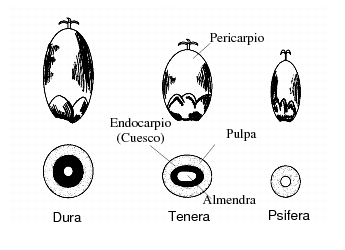
\includegraphics[scale=1]{../figures/figura.png}
\caption{Tipos y partes de la semilla de  palma de aceite, fuente}
\cite{AG03p,AG04p}
\end{figure}





\section{Citación de tablas y cuadros}
%\markboth{}{}

Para la edición de tablas, cada columna debe llevar su título; la primera palabra se debe escribir con mayúscula inicial y preferiblemente sin abreviaturas. En las tablas y cuadros, los títulos y datos se deben ubicar entre líneas horizontales y verticales cerradas.\\

La numeración de las tablas se realiza de la misma manera que las figuras o ilustraciones, a lo largo de todo el texto. Deben llevar un título breve, que concreta el contenido de la tabla; éste se debe escribir en la parte superior de la misma. Para la presentación de cuadros, se deben seguir las indicaciones dadas para las tablas.\\

Un ejemplo para la presentación y citación de tablas (citación indirecta), se presenta a continuación:

De esta participación aproximadamente el 60 \% proviene de biomasa (ver Tabla 2 1).\\

\begin{table}[h]
\centering
\begin{tabular}{|l|c|c|} 
\hline
\multirow{2}{*}{Región} & \multicolumn{2}{l|}{Participación de suministros de energía primaria}                                                                 \\ 
\cline{2-3}
                        & \begin{tabular}[c]{@{}c@{}}Energías \\Renovables\end{tabular} & \begin{tabular}[c]{@{}c@{}}Participación\\de la biomasa\end{tabular}  \\ 
\hline
Latinoamerica           & 28,9                                                          & 62,4                                                                  \\ 
\hline
Colombia                & 27,7                                                          & 54,4                                                                  \\ 
\hline
Alemania                & 3,8                                                           & 65,8                                                                  \\ 
\hline
Mundial                 & 13,1                                                          & 79,4                                                                  \\
\hline
\end{tabular}
\caption{Participación de las energías renovables primarias, fuente.}
\end{table}

\subsection{Consideraciones adicionales para el manejo de figuras y tablas}

Cuando una tabla o cuadro ocupa más de una página, se debe repetir su identificación numérica, seguida por la palabra continuación, con mayúscula inicial, entre paréntesis, como el siguiente ejemplo.\\

\textbf{Tabla 1-1:} 	(Continuación)

Adicional mente los encabezados de las columnas se deben repetir en todas las páginas después de la primera. 

\begin{itemize}
\item Ejemplo de presentación y citación de ecuaciones
\end{itemize}  

Un ejemplo para la presentación y citación de ecuaciones, se presenta a continuación: … de esta forma, el punto de partida es una ecuación de velocidad, independiente de los cambios a nivel interno del carbonizado que afectan la reacción, constituida por dos términos dependientes de la temperatura de gasificación y del medio gasificante, respectivamente, y a su vez independientes entre sí (ver Ecuación (2.1)).

\begin{equation}
-r=-\frac{dW_C/dt}{W_C}=f\left(T_G\right).f(C_{H_2O})
\end{equation}

Para el manejo de cifras y siglas, oriéntese por el Sistema Internacional de Medidas (mayor información en http://www.sc.ehu.es)\\ 

Sólo refiera las fuentes de tablas y figuras, si estás corresponden a un origen diferente al trabajo de los autores del estudio que se reporta, o si han sido adaptadas de una fuente externa. \\

Puede utilizar colores a la escala de grises, sólo en los casos que las figuras así lo demanden para comprensión de contenido. También puede utilizar un sombreado suave en los encabezados de tablas, para distinguirlos de su contenido. En todo caso, el estilo que utilice en las tablas, debe ser el mismo en todos los capítulos.\\ 

En el caso de figuras resultantes de análisis estadísticos o similares, deben quedan debidamente identificados: significado de ejes, unidades de medida, nombre de series, horizonte de tiempo (si aplica).\\

